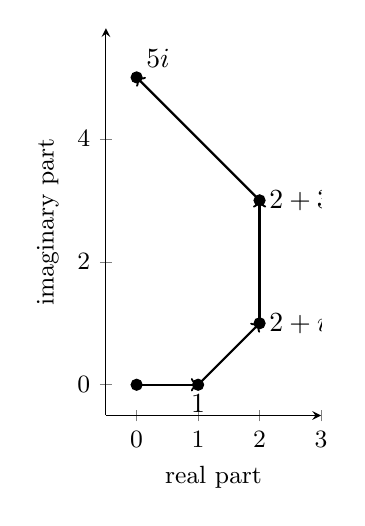
\begin{tikzpicture}
\begin{axis}[width=11cm,height=6.5cm,axis lines=left,tick label style={font=\small},label style={font=\small},legend style={font=\scriptsize},xlabel={real part},ylabel={imaginary part},xmin=-0.5,xmax=3,ymin=-0.5,ymax=5.8,axis equal image]
\addplot[black,only marks,mark=*] coordinates {(0,0)(1,0)(2,1)(2,3)(0,5)};
\node[above right] at (axis cs:0,5) {$5i$};\node[below] at (axis cs:1,0) {$1$};\node[right] at (axis cs:2,1) {$2+i$};\node[right] at (axis cs:2,3) {$2+3i$};
\draw[->,thick] (axis cs:0,0)--(axis cs:1,0);\draw[->,thick] (axis cs:1,0)--(axis cs:2,1);\draw[->,thick] (axis cs:2,1)--(axis cs:2,3);\draw[->,thick] (axis cs:2,3)--(axis cs:0,5);\end{axis}\end{tikzpicture}
